\documentclass{report}
\usepackage[utf8]{inputenc}
\usepackage{booktabs}
\usepackage{graphicx}
\usepackage[english]{babel}
\usepackage{hyperref}
\usepackage{enumitem}
\usepackage[backend=biber,style=verbose-trad2, citestyle=numeric]{biblatex}
\usepackage{listings, xcolor}
\usepackage[yyyymmdd]{datetime}
\renewcommand{\dateseparator}{.}
\addbibresource{citations/assignement2.bib}
\lstset{
tabsize = 4, %% set tab space width
showstringspaces = false, %% prevent space marking in strings, string is defined as the text that is generally printed directly to the console
numbers = left, %% display line numbers on the left
commentstyle = \color{green}, %% set comment color
keywordstyle = \color{blue}, %% set keyword color
stringstyle = \color{red}, %% set string color
rulecolor = \color{black}, %% set frame color to avoid being affected by text color
basicstyle = \small \ttfamily , %% set listing font and size
breaklines = true, %% enable line breaking
numberstyle = \tiny,
}
\newlist{parlist}{enumerate}{1}
\setlist[parlist]{label=(\alph*),wide=0pt,topsep=0pt}


\begin{document}
\begin{center}
    
\end{center}
    \begin{figure}[htb]
            \centering
\includegraphics[width=.5\textwidth]{Immagini/FUlogo.png}
    \end{figure}
    

 {\centering\scshape\LARGE\bfseries Aufgabe 2
    \begin{center}
	   Tim Neutze \\  5578777 \\
       Lorenzo Tecchia \\ 5581906  \\ \today
    \end{center}}


    \newpage
    
    \tableofcontents
    \listoffigures
    
    \chapter{Task 1}
\section{c)}
\begin{center}
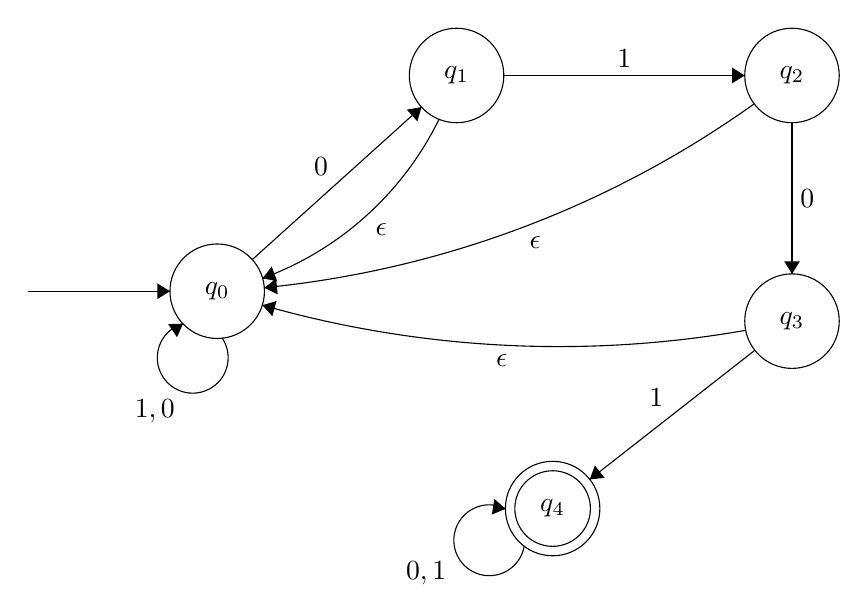
\begin{tikzpicture}[scale=0.2]
\tikzstyle{every node}+=[inner sep=0pt]
\draw [black] (13,-36.1) circle (3);
\draw (13,-36.1) node {$q_0$};
\draw [black] (28.2,-22.4) circle (3);
\draw (28.2,-22.4) node {$q_1$};
\draw [black] (49.5,-22.4) circle (3);
\draw (49.5,-22.4) node {$q_2$};
\draw [black] (49.5,-38) circle (3);
\draw (49.5,-38) node {$q_3$};
\draw [black] (34.3,-49.9) circle (3);
\draw (34.3,-49.9) node {$q_4$};
\draw [black] (34.3,-49.9) circle (2.4);
\draw [black] (1,-36.1) -- (10,-36.1);
\fill [black] (10,-36.1) -- (9.2,-35.6) -- (9.2,-36.6);
\draw [black] (15.23,-34.09) -- (25.97,-24.41);
\fill [black] (25.97,-24.41) -- (25.04,-24.57) -- (25.71,-25.32);
\draw (19.59,-28.76) node [above] {$0$};
\draw [black] (31.2,-22.4) -- (46.5,-22.4);
\fill [black] (46.5,-22.4) -- (45.7,-21.9) -- (45.7,-22.9);
\draw (38.85,-21.9) node [above] {$1$};
\draw [black] (49.5,-25.4) -- (49.5,-35);
\fill [black] (49.5,-35) -- (50,-34.2) -- (49,-34.2);
\draw (50,-30.2) node [right] {$0$};
\draw [black] (27.085,-25.182) arc (-26.08581:-69.85652:20.23);
\fill [black] (15.88,-35.28) -- (16.81,-35.47) -- (16.46,-34.53);
\draw (23.42,-31.8) node [below] {$\epsilon$};
\draw [black] (47.14,-39.85) -- (36.66,-48.05);
\fill [black] (36.66,-48.05) -- (37.6,-47.95) -- (36.98,-47.16);
\draw (40.89,-43.45) node [above] {$1$};
\draw [black] (32.495,-52.281) arc (-9.43495:-297.43495:2.25);
\draw (27.57,-54.03) node [left] {$0,1$};
\fill [black] (31.31,-49.92) -- (30.6,-49.29) -- (30.44,-50.28);
\draw [black] (46.557,-38.583) arc (-80.04686:-105.9128:68.658);
\fill [black] (15.87,-36.99) -- (16.5,-37.69) -- (16.77,-36.72);
\draw (31.07,-40.07) node [below] {$\epsilon$};
\draw [black] (47.1,-24.2) arc (-54.47005:-84.38345:64.373);
\fill [black] (15.99,-35.88) -- (16.84,-36.3) -- (16.74,-35.3);
\draw (33.2,-32.6) node [below] {$\epsilon$};
\draw [black] (13.315,-39.072) arc (33.77514:-254.22486:2.25);
\draw (9.04,-42.98) node [below] {$1,0$};
\fill [black] (10.83,-38.16) -- (9.89,-38.19) -- (10.45,-39.02);
\end{tikzpicture}
\end{center}

\section{d)}
\begin{center}
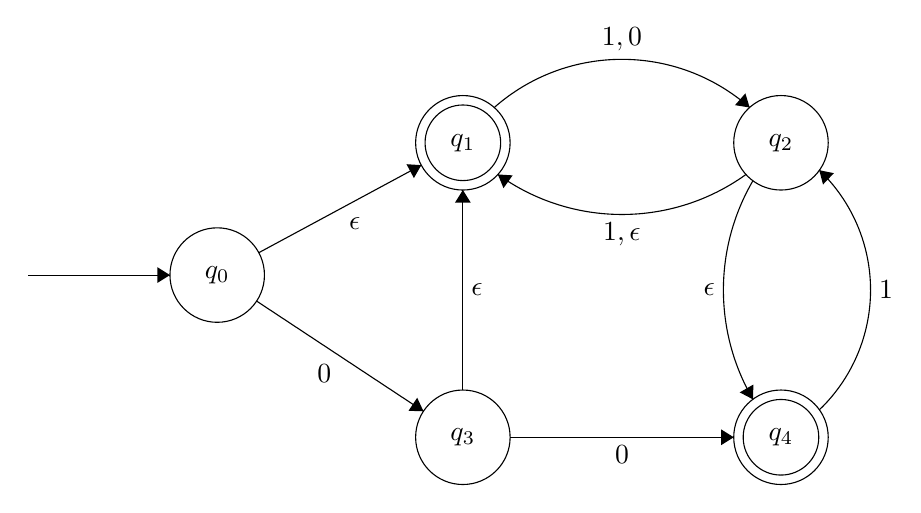
\begin{tikzpicture}[scale=0.2]
\tikzstyle{every node}+=[inner sep=0pt]
\draw [black] (15.5,-30) circle (3);
\draw (15.5,-30) node {$q_0$};
\draw [black] (31.1,-21.6) circle (3);
\draw (31.1,-21.6) node {$q_1$};
\draw [black] (31.1,-21.6) circle (2.4);
\draw [black] (51.3,-21.6) circle (3);
\draw (51.3,-21.6) node {$q_2$};
\draw [black] (51.3,-40.3) circle (3);
\draw (51.3,-40.3) node {$q_4$};
\draw [black] (51.3,-40.3) circle (2.4);
\draw [black] (31.1,-40.3) circle (3);
\draw (31.1,-40.3) node {$q_3$};
\draw [black] (3.5,-30) -- (12.5,-30);
\fill [black] (12.5,-30) -- (11.7,-29.5) -- (11.7,-30.5);
\draw [black] (18.14,-28.58) -- (28.46,-23.02);
\fill [black] (28.46,-23.02) -- (27.52,-22.96) -- (27.99,-23.84);
\draw (24.24,-26.3) node [below] {$\epsilon$};
\draw [black] (33.088,-19.363) arc (131.37205:48.62795:12.274);
\fill [black] (49.31,-19.36) -- (49.04,-18.46) -- (48.38,-19.21);
\draw (41.2,-15.8) node [above] {$1,0$};
\draw [black] (49.081,-23.609) arc (-54.21729:-125.78271:13.478);
\fill [black] (33.32,-23.61) -- (33.68,-24.48) -- (34.26,-23.67);
\draw (41.2,-26.65) node [below] {$1,\epsilon$};
\draw [black] (49.52,-37.893) arc (-149.75091:-210.24909:13.782);
\fill [black] (49.52,-37.89) -- (49.55,-36.95) -- (48.68,-37.45);
\draw (47.14,-30.95) node [left] {$\epsilon$};
\draw [black] (18,-31.65) -- (28.6,-38.65);
\fill [black] (28.6,-38.65) -- (28.2,-37.79) -- (27.65,-38.62);
\draw (22.3,-35.65) node [below] {$0$};
\draw [black] (34.1,-40.3) -- (48.3,-40.3);
\fill [black] (48.3,-40.3) -- (47.5,-39.8) -- (47.5,-40.8);
\draw (41.2,-40.8) node [below] {$0$};
\draw [black] (53.733,-23.337) arc (46.31037:-46.31037:10.528);
\fill [black] (53.73,-23.34) -- (53.97,-24.25) -- (54.66,-23.53);
\draw (57.49,-30.95) node [right] {$1$};
\draw [black] (31.1,-37.3) -- (31.1,-24.6);
\fill [black] (31.1,-24.6) -- (30.6,-25.4) -- (31.6,-25.4);
\draw (31.6,-30.95) node [right] {$\epsilon$};
\end{tikzpicture}
\end{center}
    \chapter{Task2}
    
    \chapter{Task 3}
	\chapter{Task 8 (c)}
If the positive integers and decimal would be represented by the formal alphabet of $\Sigma = {0,1}$ with 1 being the positive integers and 0 being the decimals, then the sum would be described by:
$$1^*0^* \cup 1^*0^*$$
    
    \printbibliography
    
\end{document}
